\documentclass{article}
\usepackage{xcolor}
\usepackage{amsmath}
\usepackage{amssymb}
\usepackage{tikz, calc}
\usetikzlibrary{calc}

\begin{document}

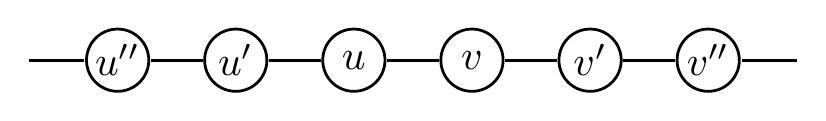
\begin{tikzpicture}[scale=1.5, every node/.style={circle, draw, scale=1.5, line width=1pt, minimum size=15pt, inner sep=0pt}]
      \node (1) at (1,0) {$u''$};
      \node (2) at (2,0) {$u'$};
      \node (3) at (3,0) {$u$};
      \node (4) at (4,0) {$v$};
      \node (5) at (5,0) {$v'$};
      \node (6) at (6,0) {$v''$};
      
      \draw [line width=1pt] (0.25,0) -- (1) -- (2) -- (3) -- (4) -- (5) -- (6) -- (6.75,0);
  \end{tikzpicture}

\end{document}